\documentclass{beamer}

\mode<presentation>

\title{Music Similarity}
\subtitle{Flash Presentation}
\author{Ali Bektas \and Paul Kröger}

\usepackage{graphicx}
\graphicspath{{./images/}}
\usepackage{verbatim}

\begin{document}
	\begin{frame}
		\maketitle
	\end{frame}
	\begin{frame}
  		\frametitle{Was wir machen}
  		\begin{itemize}
  			\item Symbolic Melodic Music Similarity 
  			\begin{itemize}
  				\item "symbolisch" heißt : Darstellung von Noten.
  				\item verschiedene Representationsansätze von Melodien 
  			\end{itemize} 
			\item Nach \cite{two} : 3 grundlegende Klassen von Algorithmen : diejenigen ,
			\begin{itemize}
				\item die Mathematik einsetzen
				\item die musiktheoretische und
				\item die kognitivwissenschaftliche Ansätze verfolgen .
			\end{itemize}
			\item und hybride Methoden(\textit{lineare Kombination} von Algorithmen).
  		\end{itemize}
	\end{frame}
	\begin{frame}
  		\frametitle{Wie man es macht}
  		\begin{figure}[h!]
					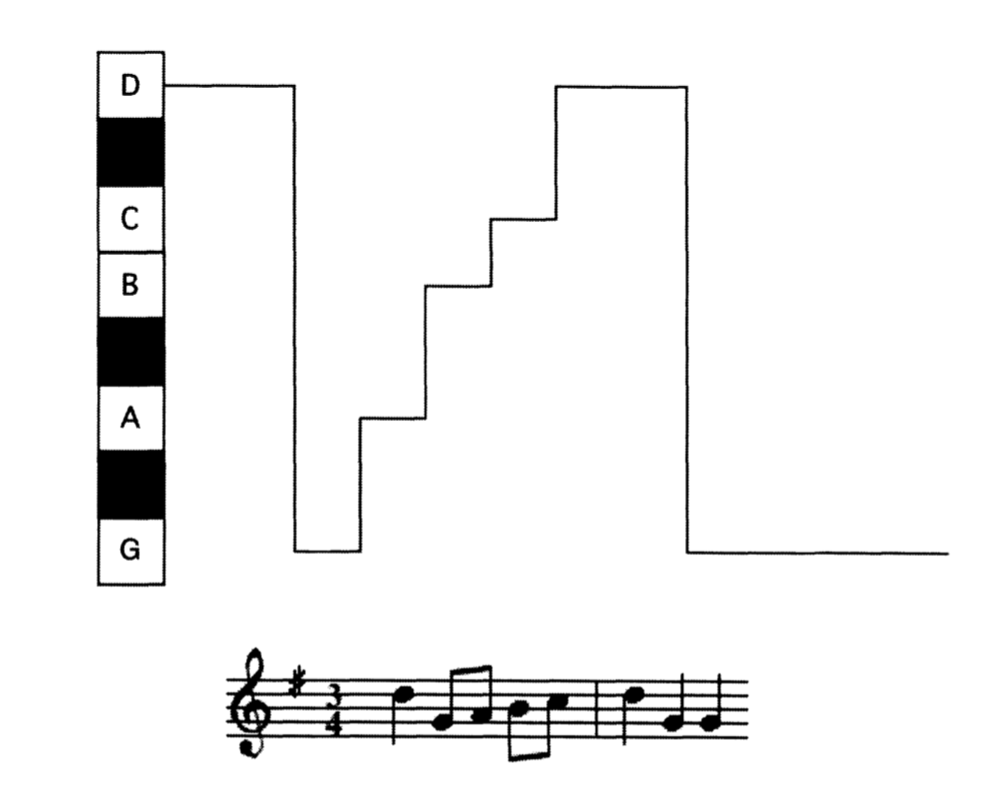
\includegraphics[width=300px,height=100px,keepaspectratio]{abb_1}
		\end{figure}
		\begin{figure}[h!]
					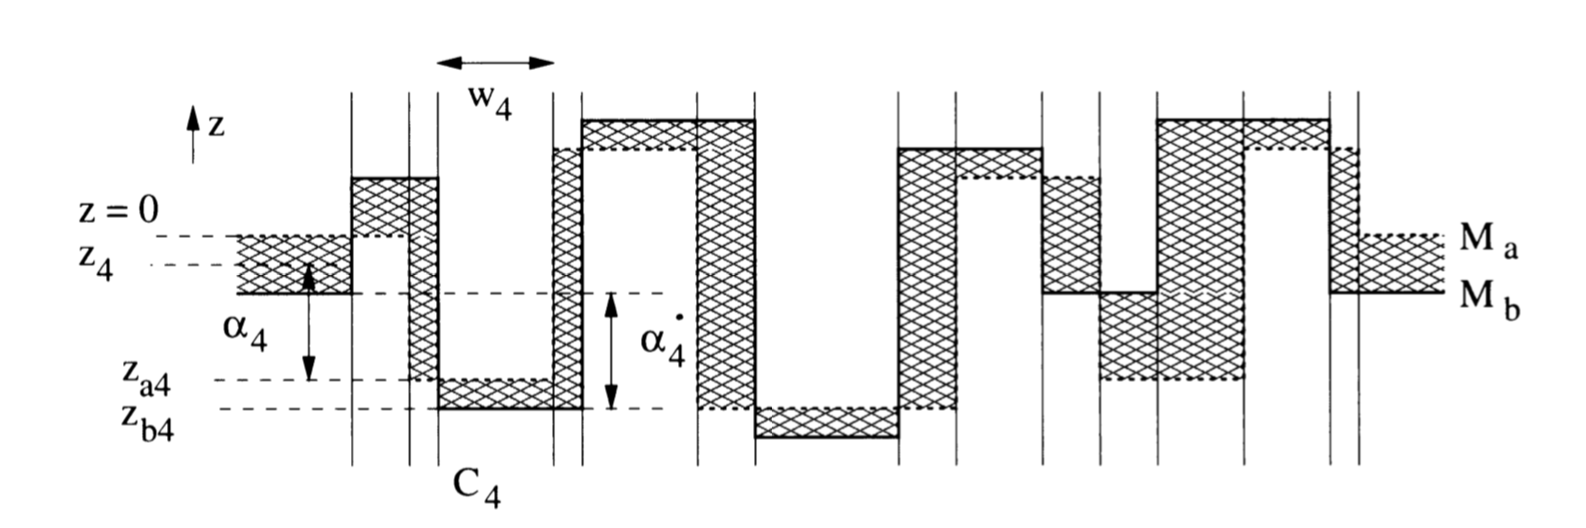
\includegraphics[width=300px,height=100px,keepaspectratio]{abb_2}
					\caption{Source: \cite{one}}
		\end{figure}
	\end{frame}
	\begin{frame}
		\frametitle{Wie man es macht}
		\begin{figure}[h!]
					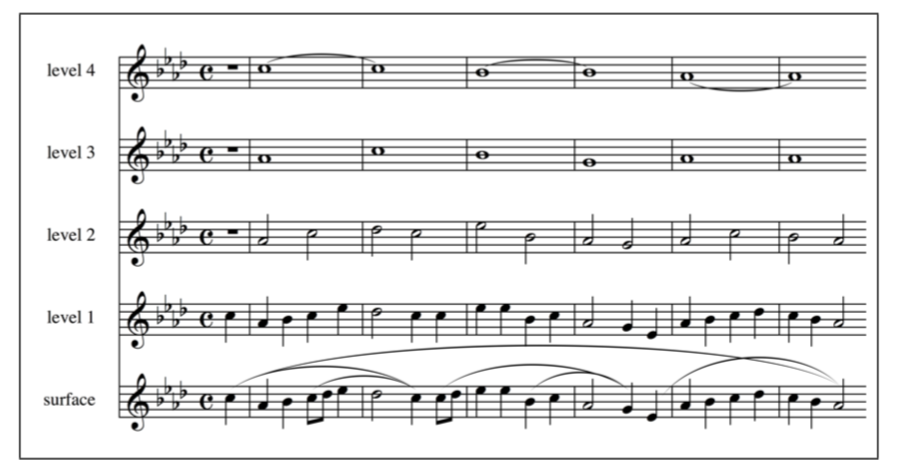
\includegraphics[width=300px,height=100px,keepaspectratio]{one_of_two_point_four}
		\end{figure}
		\begin{figure}[h!]
					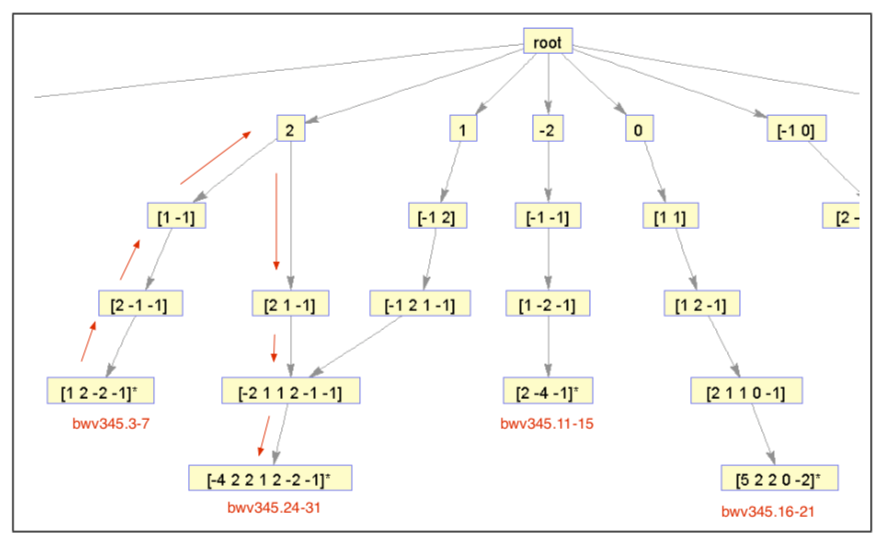
\includegraphics[width=300px,height=100px,keepaspectratio]{two_of_two_point_four}
					\caption{Source: \cite{two_point_four}}

		\end{figure}
	\end{frame}
	\begin{frame}
		\frametitle{Wie man es macht}
		\begin{figure}[h!]
					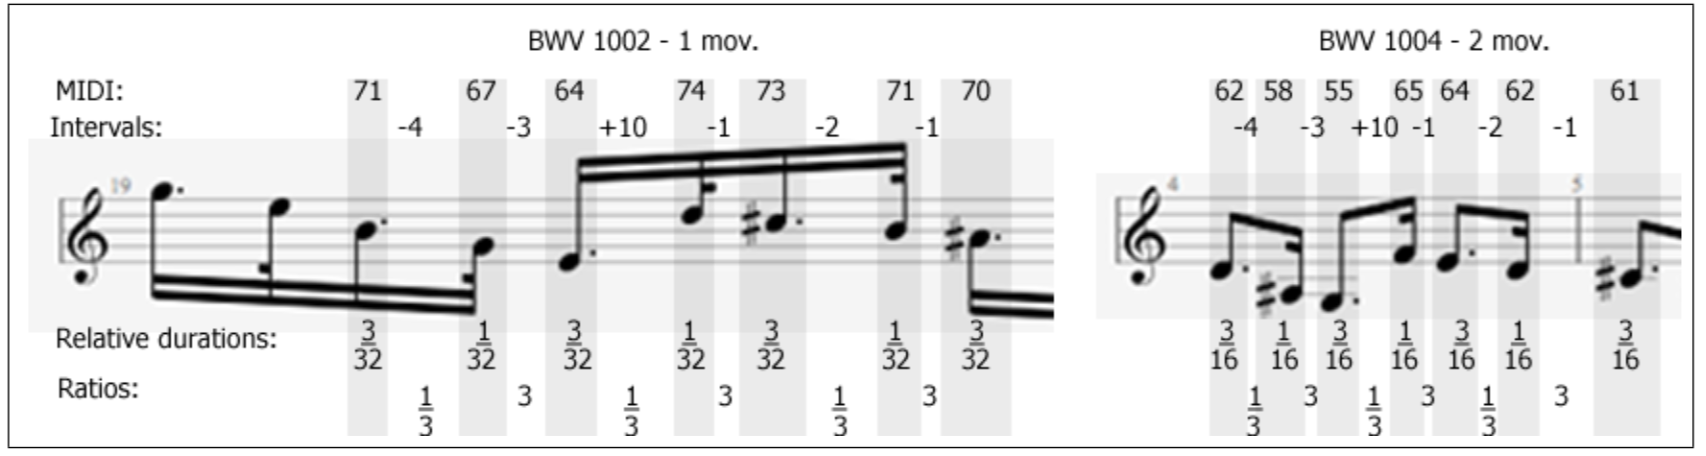
\includegraphics[width=300px,height=100px,keepaspectratio]{one_of_two_point_seven}
					\caption{Source: \cite{two_point_seven}}
		\end{figure}
	\end{frame}


	\begin{frame}
		\begin{thebibliography}{9}
			\setbeamertemplate{bibliography item}[text]
			\bibitem[1]{two} "Algorithms for Computing Geometric Measures of  Melodic Similarity" , G.Aloupis,T.Fevens,S.Langerman,T.Matsui,A.Mesa, Y. Nufiez, D. Rappaport, G. Toussaint. Computer Music Journal , 30:3, pp. 67-76, Fall 2006.
			\bibitem[2]{one} "Downie J.S., Ehmann A.F., Bay M., Jones M.C. (2010) The Music Information Retrieval Evaluation eXchange: Some Observations and Insights. In: Raś Z.W., Wieczorkowska A.A. (eds) Advances in Music Information Retrieval. Studies in Computational Intelligence, vol 274. Springer, Berlin, Heidelberg"
			\bibitem[3]{two_point_four} Orio, N., and A. Roda`. 2009. “A Measure of Melodic Similarity Based on a Graph Representation of the Music Structure.” In Proceedings of the International Conference for Music Information Retrieval, pp. 543– 548.
			\bibitem[4]{two_point_seven} de Carvalho, A. D., Jr., and L. V. Batista. 2012. “SMS Identification Using PPM, Psychophysiological Concepts, and Melodic and Rhythmic Elements.” In Proceedings of the Annual Music Information Retrieval Evaluation Exchange.
		\end{thebibliography}
	\end{frame}
\end{document}